\RequirePackage[l2tabu, orthodox, abort]{nag}
\documentclass[a4paper, 11pt]{article}

\usepackage[utf8x]{inputenc}
\usepackage[T1]{fontenc}
\usepackage{ucs}
\usepackage[english]{babel}
\usepackage{mathtools, amsmath, amsfonts, amssymb}
\usepackage{fancyhdr}
\usepackage{graphicx}
\usepackage[sc]{mathpazo}
\usepackage[scaled]{beramono}
\usepackage[scaled]{helvet}
\usepackage{float}
\usepackage[font={small,it}]{caption}
\usepackage{fixltx2e}
\usepackage{bm}
\usepackage{fullpage}
\usepackage{verbatim}
\usepackage{subcaption}
\usepackage[noabbrev]{cleveref}
\usepackage{booktabs}
\usepackage{xfrac}
% \usepackage[parfill]{parskip}

\linespread{1.05}
\pagestyle{fancyplain}
\fancyhead{}
\fancyfoot[L]{}
\fancyfoot[C]{}
\fancyfoot[R]{\thepage}
\renewcommand{\headrulewidth}{0pt}
\renewcommand{\footrulewidth}{0pt}
\setlength{\headheight}{13.6pt}

\widowpenalty=9000
\clubpenalty=9000

\newcommand{\horrule}[1]{\rule{\linewidth}{#1}}
\newcommand{\vect}[1]{\mathbf{#1}}
\newcommand{\mat}[1]{\textbf{#1}}

% Todonotes commands.
\newcommand{\addref}{\todo[color=red!40]{Add reference.}}
\newcommand{\rewrite}[1]{\todo[color=green!40]{#1}} 
\newcommand{\missing}[1]{\todo[inline,color=green!40]{Need to write: #1}}

\title{ 
\normalfont\normalsize 
\textsc{University of Copenhagen} \\ [25pt]
\horrule{0.5pt} \\[0.4cm]
\huge StatML\@: Exam 2014\\
\horrule{2pt} \\[0.5cm]
}

\author{Jens Fredskov (chw752)}

\begin{document}
\maketitle
\pagebreak

\section{Predicting the Specific Star Formation Rate} % (fold)
\label{sec:predicting_the_specific_star_formation_rate}

\subsection*{Question 1}
For this question a maximum likelihood linear regression has been used. This means the basis functions used were linear such that $\phi_j(\mathbf{x}) = x_j$, except for the first function which were $\phi_0(\mathbf{x}) = 1$, as this is a dummy function to allow a bias. When applying the maximum likelihood method\footnote{This is simply using $\mathbf{w}_{\mathit{ML}} = \bm\Phi^\dagger t$, where $\bm\Phi^\dagger$ is the Moore-Penrose pseudo-inverse of $\bm\Phi$ and $t$ is the target of our data.} using a classic design matrix $\bm\Phi$ constructed from the basis functions and the data from the training set, I got a weight vector
\[
    \mathbf{w}_{\mathit{ML}} = \begin{pmatrix}
      -8.1494 \\
       -0.794 \\
       -1.223 \\
     -0.32858 \\
     -0.78633 \\
    \end{pmatrix}
    \label{eq:wml}
\]
which when applied to the data gave mean squared errors of
\begin{align*}
    \mathrm{MSE}_{\mathit{train}} &= 0.27475 \\
    \mathrm{MSE}_{\mathit{test}} &= 0.27518
\end{align*}

The error of the two sets is almost equal, which suggests that we probably have not over-fitted to the training data. Furthermore the error is reasonably small, leading to the conclusion that a linear model, might be a good choice of model for our data.

The source code used in the implementation of this question can be found in \texttt{question1.m}, \texttt{linearRegression.m} and \texttt{meanSquaredError.m}.

\subsection*{Question 2}
For the non-linear regression I initially decided to perform a maximum likelihood polynomial regression. However as the results left a lot to be desired, I also trained a feed-forward neural network, using resilient back-propagation.

The maximum likelihood polynomial regression was implemented in the following way. As in the linear case I created a design matrix $\bm\Phi$. The basis functions however were defined as
\[
    \phi_j(\mathbf{x}) = \sum_{i=1}^{n-1} x_i^j, \quad
    \mathbf{x} = \begin{pmatrix}
        x_1 \\ x_2 \\ \vdots \\ x_n
    \end{pmatrix} \; \wedge \; 0 < j \le m
\]
were $m$ is the size of the polynomial and $\mathbf{x}$ is a data point of $n$ dimensions, including the target as the $n$th dimension. As in the linear case to allow a bias the first basis funtion $\phi_0(\mathbf{x}) = 1$. Using these I created the classic design matrix
\[
    \bm\Phi = \begin{pmatrix}
        \phi_0(\mathbf{x}_1) & \phi_1(\mathbf{x}_1) & \cdots & \phi_m(\mathbf{x}_1) \\
        \phi_0(\mathbf{x}_2) & \phi_1(\mathbf{x}_2) & \cdots & \phi_m(\mathbf{x}_2) \\
        \vdots & & & \vdots \\
        \phi_0(\mathbf{x}_N) & \phi_1(\mathbf{x}_N) & \cdots & \phi_m(\mathbf{x}_N)
    \end{pmatrix}
\]
and applied the maximum likelihood method as in the linear case, using the Moore-Penrose pseudo-inverse. However in this case there was a hyper parameter to tweak as I had to decide the degree of the polynomial. Thus the weights were found for polynomials of degree 1 to 15 and the mean squared error on these were found on the training and test data. The resulting plot can be seen in \Cref{fig:question2_1}.

\begin{figure}[H]
    \centering
    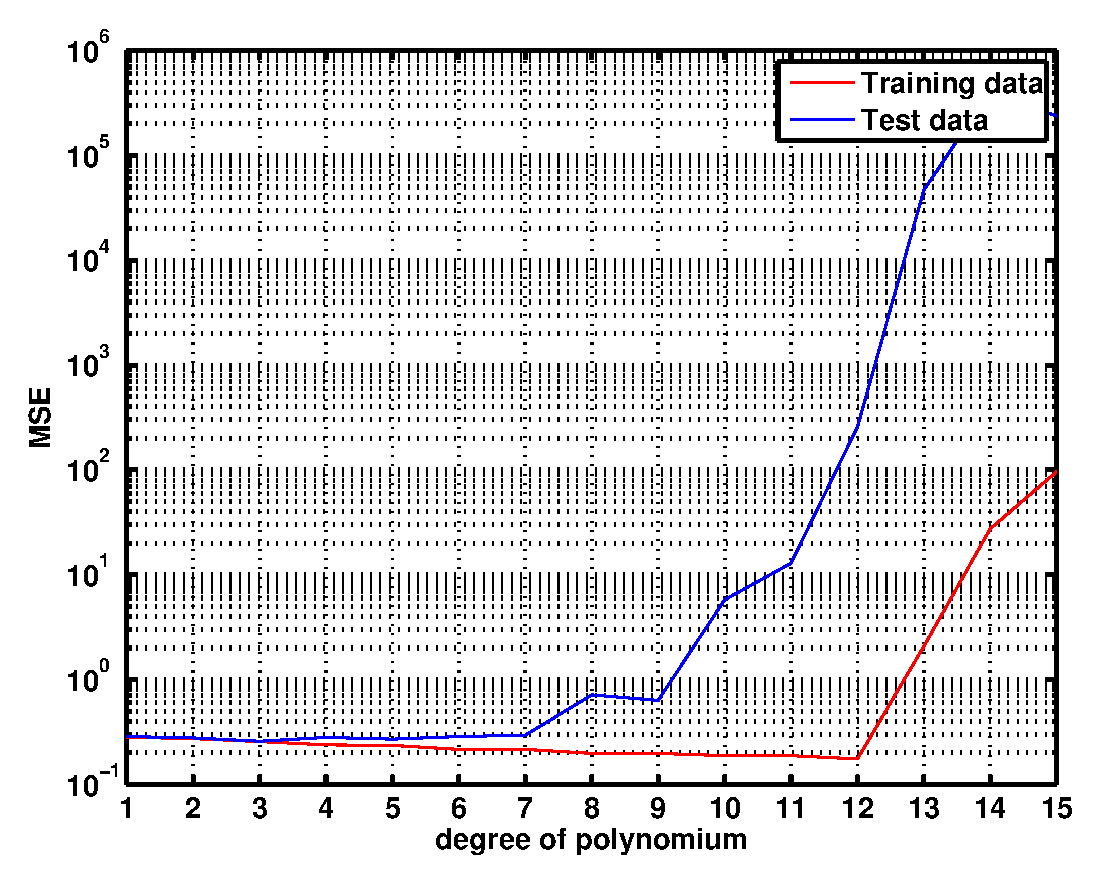
\includegraphics[width=0.5\textwidth]{figures/question2_1}
    \caption{The degree of the polynomium plotted against the mean squared error obtained on the training and test data.}\label{fig:question2_1}
\end{figure}

As can be seen in \Cref{fig:question2_1} the error of the test set started to diverge from the training data at a degree of 3. However as the hyper parameters should be chosen only based on the training data I chose a polynomial of degree 12 as this is the minimum of the training error. With a polynomial of degree 12 I got errors of
\begin{align*}
    MSE_{\mathit{train}} &= 0.17507 \\
    MSE_{\mathit{test}} &= 258.02
\end{align*}

It is clear from the big difference in error that the model have over-fitted to the training data. Furthermore when looking at any degree larger than 12 the error starts to rise exponentially (thus the need for a logarithmic scale on the y-axis) in both the test and training data. A proper polynomial regression should in theory fit better and better to the training data, and when the polynomial reached a degree corresponding to the number of data points an error of 0 should be possible. Thus the results leaves me to conclude that not only  is this model probably not a good choice for the data, it also does not seem to be a proper polynomial regression, at least not in the classic sense.

To try and achieve better general performance regularisation could have been used. Another alternative would be to use other basis functions like `Gaussian' or sigmoidal basis functions. The regularisation I decided not to do as the polynomial regression seemed to be wrong, thus I decided the time would be better spent on trying out a neural network instead. I decided against trying other basis functions, as we during the lectures have not seen examples of using these with more than one dimension in the input\footnote{This actually also applies to the polynomial basis functions, and maybe I should have decided against trying to model them on that basis alone.}.

Because of the result of the maximum likelihood polynomial regression I also tried a feed-forward neural network. The implementation widely uses MATLABs neural network toolbox. The network created uses a standard hyperbolic tangent sigmoid function as the activation function for the hidden layer, a linear transfer function for the output neuron, and a single hidden layer with 1 to 100 neurons. To train the network the implementation uses resilient back-propagation.

Most of the the standard settings for the network were kept, but for the training of the network the training data is split so 70\% is used for training, 15\% for validation and 15\% for test.

The error when applying the trained network on training and test data can be seen in \Cref{fig:question2_2}.

\begin{figure}[H]
    \centering
    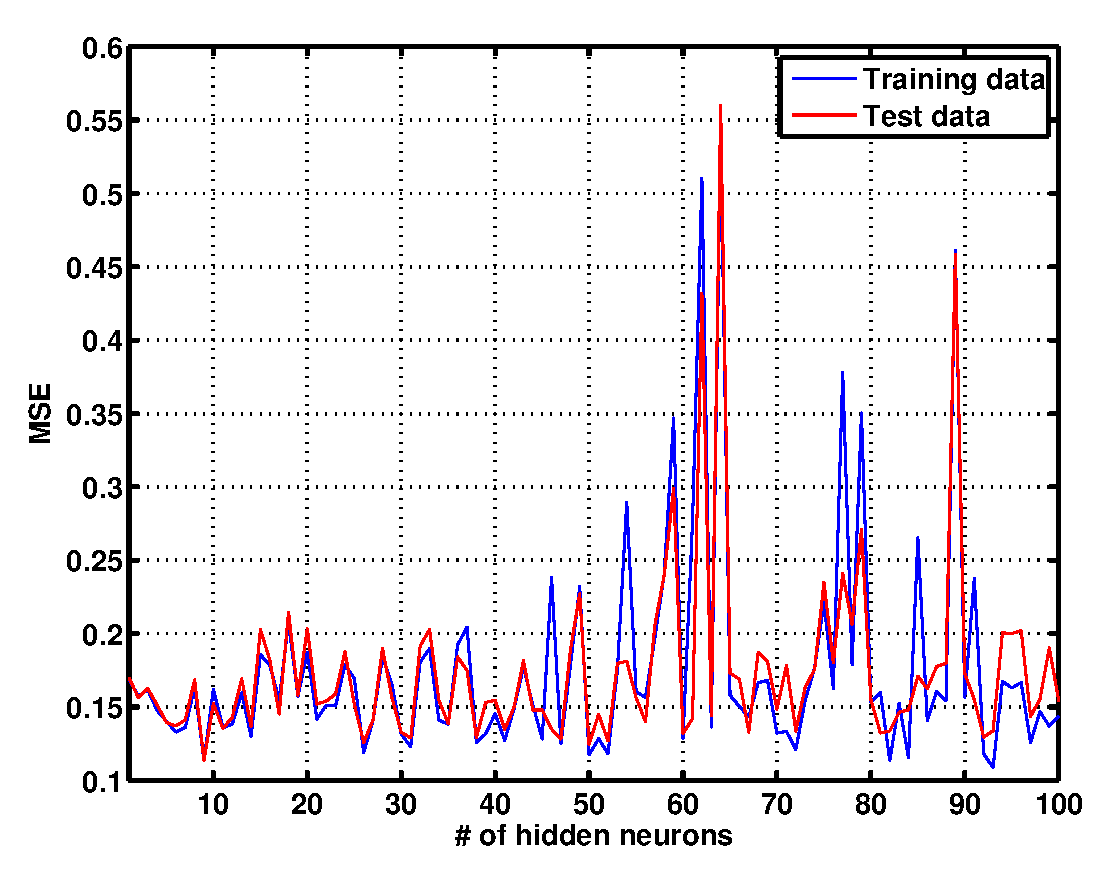
\includegraphics[width=0.5\textwidth]{figures/question2_2}
    \caption{The number of hidden neurons plotted against the mean squared error obtained on the training and test data. As can be seen the error fluctuates a lot.}\label{fig:question2_2}
\end{figure}

As can be seen the error fluctuated a lot, but most of the time it kept below 0.2 for both of the data sets, which is better than the linear model in question 1. The number of neurons which gave the lowest training error was 93 hidden neurons. 93 hidden neurons gave errors of
\begin{align*}
    MSE_{\mathit{train}} &= 0.10871 \\
    MSE_{\mathit{test}} &= 0.13374
\end{align*}

Both of these errors are small and close enough that it does not look like we have overfitted to the training set. We might therefore expect that the model will perform well in general on this type of data.

The source code used in the implementation of this question can be found in \texttt{question2.m}, \texttt{polyRegression.m}, \texttt{polyPredict.m}, \texttt{meanSquaredError.m} and \texttt{betterPlots.m}.

% section predicting_the_specific_star_formation_rate (end)

\section{Stars vs. Galaxies} % (fold)
\label{sec:stars_vs_galaxies}

\subsection*{Question 3}
I have made use of the \texttt{libsvm-3.17}\footnote{http://www.csie.ntu.edu.tw/\textasciitilde{}cjlin/libsvm/} library to perform the standard C-SVM binary classification.

Using the described Jaakkola's heuristic I calculated the initial value for $\sigma$ and afterwards for $\gamma$, using the identity
\[
    \sigma = \sqrt{1 / (2 \gamma)} \Leftrightarrow \gamma = 1 / (2 \sigma^2)
\]

The initial values suggested by the heuristic was
\[
    \sigma_{\mathit{jaakkola}} = 1.8119,\quad \gamma_{\mathit{jaakkola}} = 0.1523
\]

Using these I performed a grid search to determine the appropriate hyper parameters for the SVM\@. The grid search was set up such that all the given combinations was tried, for each of the three given bases. That I tried every combination of the type
\[
    \lbrace C \times \gamma \rbrace \in \lbrace b^i \times \gamma_{\mathit{jaakkola}} \cdot b^j | -2 \le i \le 3 \wedge -3 \le j \le 3 \wedge b \in \lbrace 2, e, 10 \rbrace \rbrace
\]
On every combination 5-fold cross validation was performed, and the one with the lowest average 0--1 loss was then chosen to be the best hyper parameters. The cross validation splits the data into the five folds by sorting the data on class and then evenly distributing the using modulo (such that every fold gets one of the first five data points, one of the five next, and so on). This is done to ensure that every fold is representative of the entire data set.

Using this method the hyper parameters was found to be
\[
    C = 1000 \quad \gamma = 0.001523
\]
with a base of $10$, so $C = 10^3$ and $\gamma = \gamma_{\mathit{jaakkola}} \cdot 10^{-2}$.

These hyper parameters and the training data were then used to train the SVM\@. The classification error on the training and test data when using the trained SVM was then
\begin{align*}
    \mathrm{Accuracy}_{\mathit{train}} &= 0.997333 = 99.73 \% \\
    \mathrm{Accuracy}_{\mathit{test}} &= 0.996333 = 99.63 \%
\end{align*}

The source code used in the implementation of this question can be found in \texttt{question3.m}, \texttt{jaakkola.m}, \texttt{crossValidation.m} and \texttt{svmClassify.m}.

\subsection*{Question 4}
To perform the PCA I have not used any libraries (e.g.\ the built in MATLAB function \texttt{pca}). The analysis was performed by first computing the covariance matrix of the data, and then the eigenvectors and -values by using. Both of these computations can be done with built in functions \texttt{cov} and \texttt{eig} of MATLAB\@. Afterwards I simply sorted the eigenvectors, by their eigenvalue. The corresponding eigenspectrum can be seen in \Cref{fig:question4_1}. As can be seen almost all of the variance is caught by the first two principal components. 

\begin{figure}[H]
    \centering
    \begin{subfigure}[t]{0.48\textwidth}
    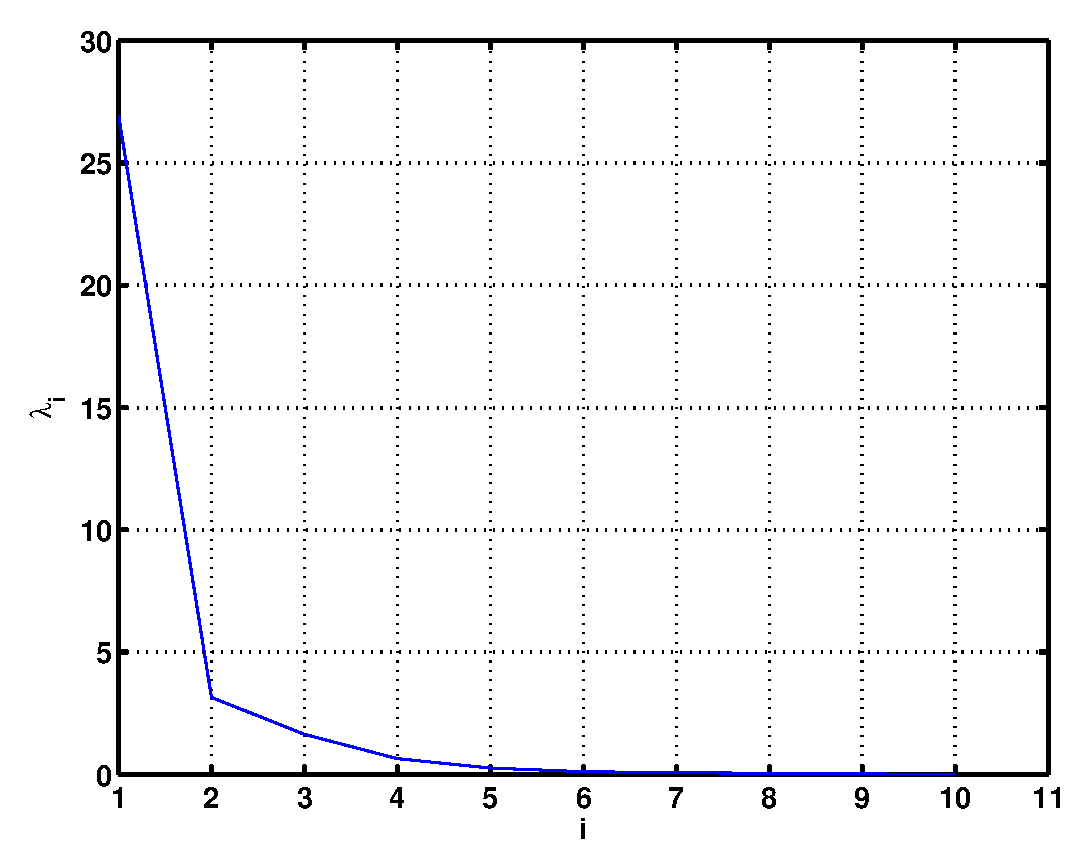
\includegraphics[width=\textwidth]{figures/question4_1}
        \caption{The eigenspectrum of the training data.}\label{fig:question4_1}
    \end{subfigure}
    \hspace{0.5em}
    \begin{subfigure}[t]{0.48\textwidth}
        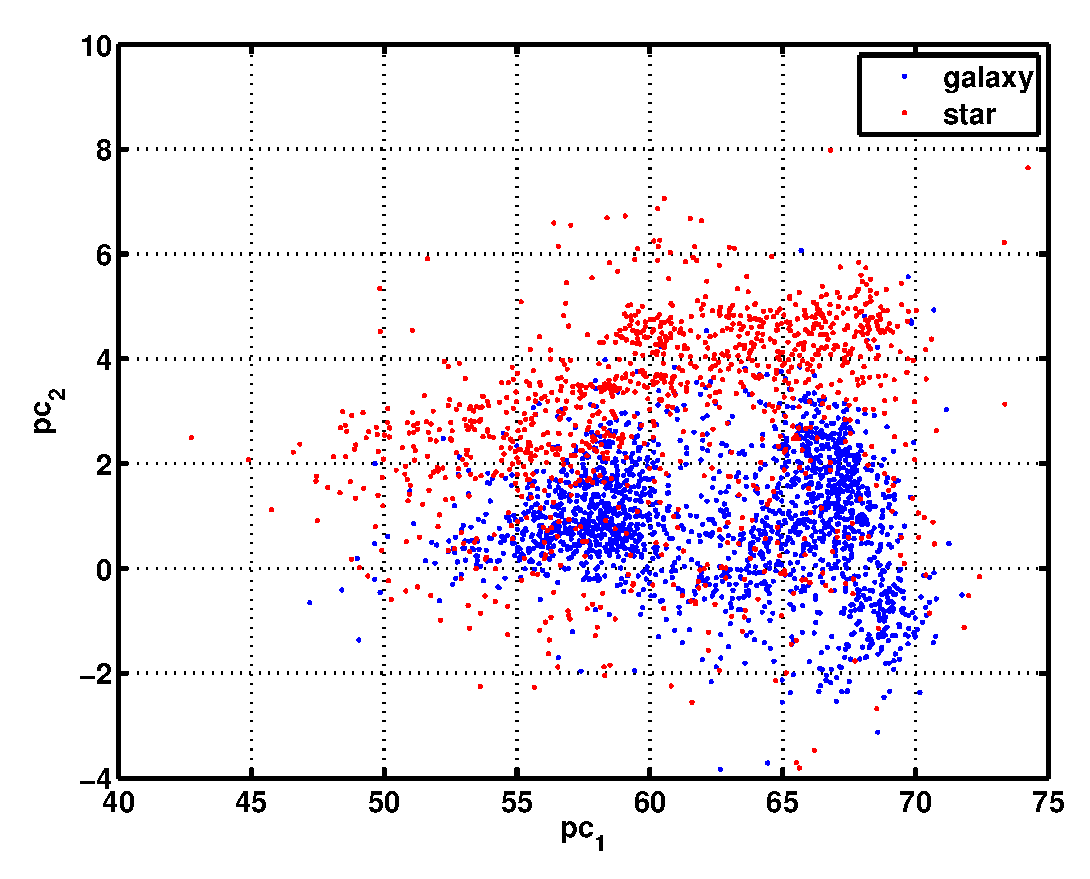
\includegraphics[width=\textwidth]{figures/question4_2}
        \caption{The training data projected on the first two principal components.}\label{fig:question4_2}
    \end{subfigure}
    \caption{Plots related to the PCA performed on the training data.}\label{fig:question4}
\end{figure}

In \Cref{fig:question4_2} the data points have been plotted after being projected on the first two principal components. As can be seen we do get a split of the two classes. However many star-class data points lie inside the galaxy-class. So while the the projection does provide at decent split, it is by no means perfect, and without the colouring of classes on might have thought the classes were divided by a horizontal line at around 62.5, as there is what seems to be a hole between two groups of points there.

The source code used in the implementation of this question can be found in \texttt{question4.m}, \texttt{pca.m} and \texttt{betterPlots.m}.

\subsection*{Question 5}
To perform the 2-means clustering I have used the built in MATLAB function \texttt{kmeans}. This function applies the iterative k-means algorithm and seeks to minimise the sum, over all clusters, of the within-cluster sums of point-to-cluster-centroid distances. The functions was set to perform 100 attempts with different starting points for the clusters. These starting points are by the function chosen as random sample points, which in general serve as better guesses than completely random points in the entire $\mathbb{R}^2$. To ensure consistent results the seed for randomisation is set beforehand (any number could be chosen, but here I have used $43786953$ which has no special meaning). The 10-dimensional centres found using this method can be found in \Cref{tab:question4}.

\begin{table}[H]
    \centering
    \begin{tabular}{lcc}
        \toprule
        Feature name & $c_1$ & $c_2$ \\
        \midrule
        cModelMag\_u & 19.324 & 22.349 \\
        cModelMag\_g & 17.971 & 21.413 \\
        cModelMag\_r & 17.291 & 20.290 \\
        cModelMag\_i & 16.965 & 19.599 \\
        cModelMag\_z & 16.774 & 19.222 \\
        psfModelMag\_u & 20.297 & 23.451 \\
        psfModelMag\_g & 18.876 & 22.096 \\
        psfModelMag\_r & 18.201 & 20.946 \\
        psfModelMag\_i & 17.880 & 20.272 \\
        psfModelMag\_z & 17.647 & 19.855 \bottomrule
    \end{tabular}
    \caption{The two 10-dimensional class centres found using 2-means clustering.}\label{tab:question4}
\end{table}

When projecting these on the first two principal components of the data its look as in \Cref{fig:question5}, where \Cref{fig:question5_1} shows the classes as guessed by the 2-means clustering and \Cref{fig:question5_2} shows the actual classes.

\begin{figure}[H]
    \centering
    \begin{subfigure}[t]{0.48\textwidth}
    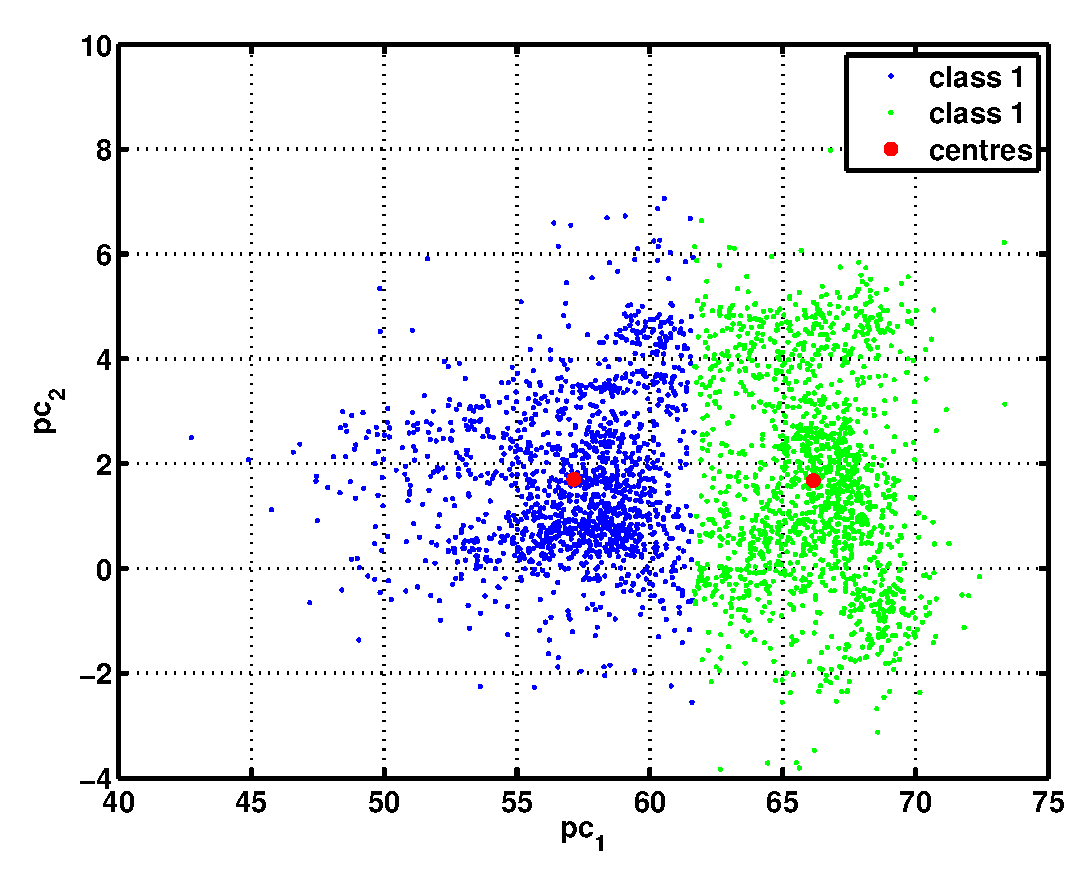
\includegraphics[width=\textwidth]{figures/question5_1}
        \caption{The projected training data and centres. Here the class colouring shows the classes as guessed by the 2-means clustering.}\label{fig:question5_1}
    \end{subfigure}
    \hspace{0.5em}
    \begin{subfigure}[t]{0.48\textwidth}
        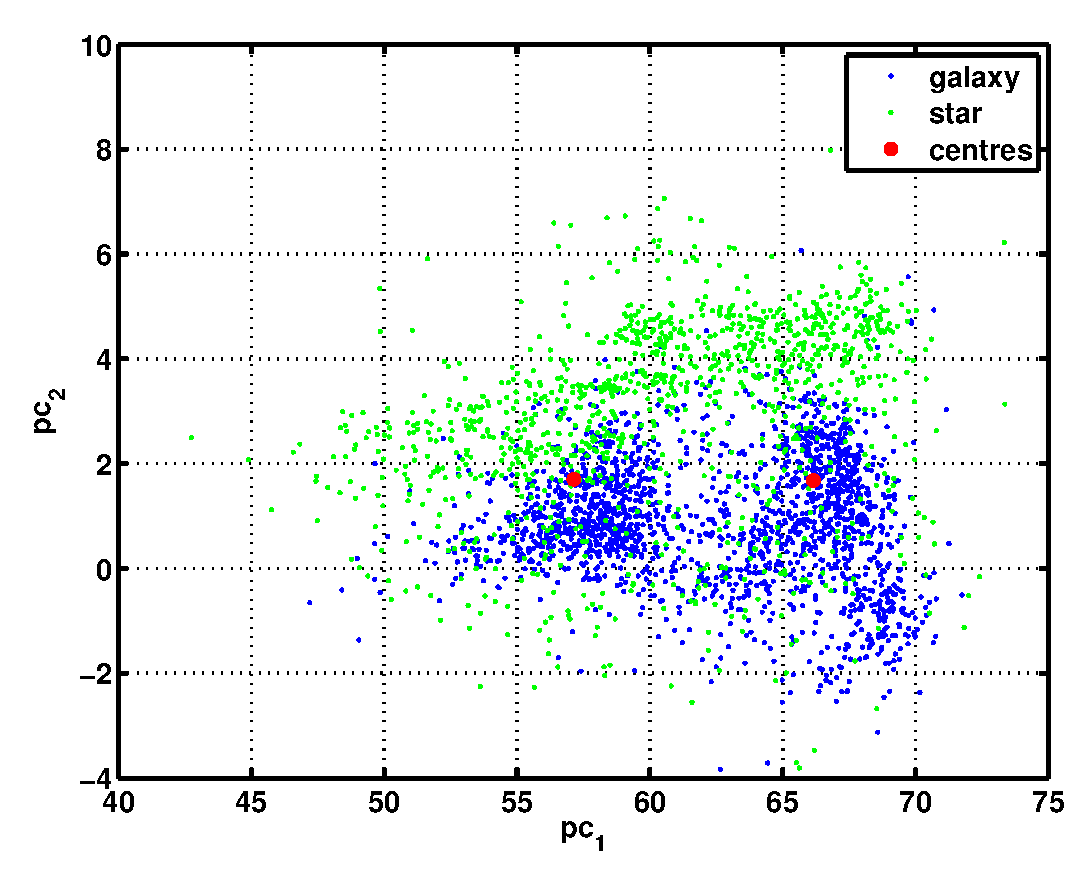
\includegraphics[width=\textwidth]{figures/question5_2}
        \caption{The projected training data and centres. Here the class colouring shows the actual classes of the training data.}\label{fig:question5_2}
    \end{subfigure}
    \caption{The projected training data and centres, show with the guessed and classes classes.}\label{fig:question5}
\end{figure}

As can be seen the 2-means clustering did not find the correct split of the two classes. The split found however makes sense, as the galaxy-class seems to be split in two clusters, with the star-class lying above. Thus it makes sense that the split was performed as seen in \Cref{fig:question5}. In general the problem with the two classes is that one is very spread out on the first axis and lies just up to the second class which lies in two compact clusters. There clusters could therefore still be seen as meaningful, as they do represent some sort of split which seem to be present in the data, but they do not represent the split between the star- and galaxy-class very well.

The source code used in the implementation of this question can be found in \texttt{question5.m} and \texttt{betterPlots.m}. Note that \texttt{question5.m} depends on \texttt{question4.m} and thus it is necessary to run this script beforehand. If the the questions are not run one at a time, but using the main script \texttt{main.m} this is already taken care of.

\subsection*{Question 6} %FIXME This has not been done yet!

% section stars_vs_galaxies (end)

\section{Variable Stars} % (fold)
\label{sec:variable_stars}

\subsection*{Question 7}

For the linear classification I decided to use linear discriminant analysis (LDA) and for the non-linear classification I used k-nearest neighbour (KNN).

I chose the LDA for the linear classification as it is simple to implement, and if there is a good linear split of the data the LDA normally performs well, as it splits using a hyperplane. Thus this seemed as a good choice for the linear classification. Furthermore LDA has no hyper parameters, so we avoid having to find these.

The KNN was chosen again firstly because the algorithm and implementation is simple. More advanced methods, e.g.\ random forests, could have been used. However this would have required significantly more time to implements as both the algorithm and required data structure is more complex. Another possibility could have been to use SVMs. We have however not covered any type of multi-class SVMs in the lectures.

To avoid having to train the LDA every time I wish to predict a point, the LDA is implemented such that it first takes the training set and then returns a function, which can predicts points using the trained model.

Running the LDA on gave errors (0--1 loss) of
\begin{align*}
    E_{\mathit{train}} &= 0.18418 = 18.418 \% \\
    E_{\mathit{test}} &= 0.28664 = 28.664 \%
\end{align*}
both of which are relatively high.

For the KNN I used the cross-validation function\footnote{It has been implemented such that it can take different models to cross-validate on, as long as it is a classification problem, as the function uses a 0--1 loss as error function. This could also have been generalised to take any error function, but has not been done.}, which I also used in question 3, to decide which $k$ to use. The cross validation was done as a 5-fold and with\footnote{This denotes all uneven integers from 1 to 120.}
\[
k \in \lbrace 1 \le 2n-1 \le 120 | n \in \mathbb{Z} \rbrace
\]
Using the cross-validation (as always we train using only the training data) $k$ was found to be
\[
    k = 5
\]
which when used with a KNN trained on the training data gave errors (0--1 loss) of
\begin{align*}
    E_{\mathit{train}} &= 0.42283 = 42.283 \% \\
    E_{\mathit{test}} &= 0.55512 = 55.512 \%
\end{align*}
both of which are very high.

Neither the LDA or the KNN gave very good results. With the LDA approximately \sfrac{1}{5} of all training data and \sfrac{1}{3} of all test data was misclassified. For the KNN the result were even worse, with a little under half of the training data and a little over half of the test data being misclassified.

As can be seen neither of the two models gave very good results. Based of the results my conclusion would be to either try different models, or to go with the linear model (LDA) as that gave the best results.

The source code used in the implementation of this question can be found in \texttt{question7.m}, \texttt{trainLDA.m}, \texttt{kNN.m} and \texttt{crossValidation.m}.

\subsection*{Question 8} %FIXME This has not been done yet!

\paragraph{Traditional over-fitting} % (fold)
\label{par:traditional_over_fitting}

% paragraph traditional_over_fitting (end)

\paragraph{Brittle measure} % (fold)
\label{par:brittle_measure}

% paragraph brittle_measure (end)

\paragraph{Human-loop over-fitting} % (fold)
\label{par:human_loop_over_fitting}

% paragraph human_loop_over_fitting (end)

% section variable_stars (end)
\end{document}